\section{Window Layout Concept}
    Developers can define their working environment to fit the needs and preferences. For a better understanding of further comments and instructions, five major screen areas are defined. % popsáno v obrázku


   \begin{figure}[h]
        \centering
        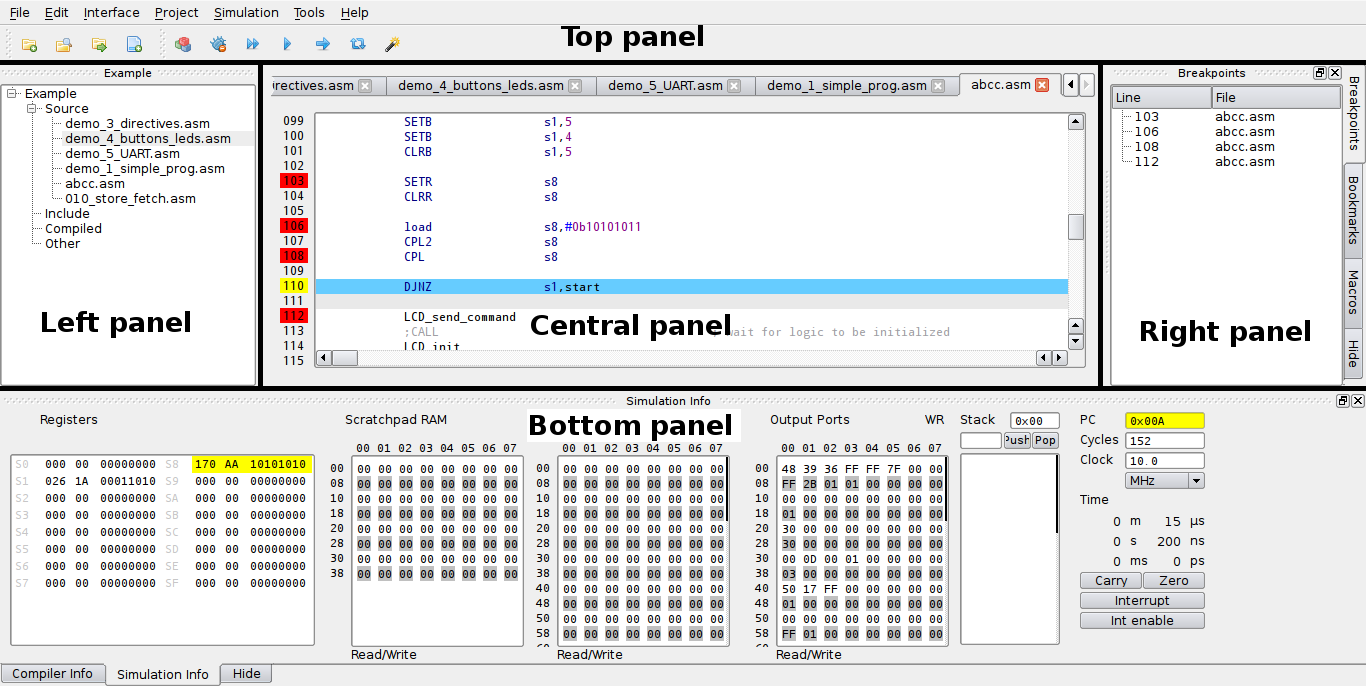
\includegraphics[width=\textwidth]{img/Main_window.png}
        \caption{Window layout concept}
    \end{figure}

\subsection{Middle panel}
    Middle panel is main text editor for writing a code. It has syntax highligh for better readability and you can easily add breakpoints and bookmarks just by clicking to desired line number.

\subsection{Top panel}
    \begin{itemize}
        \item New file: creates a new document to enter a new source file.
        \item Open file: allows to open an existing source file.
        \item Open recent: lists the 5 most recently used files.
        \item Add to project:
        \item Save file: saves the open document to the related file.
        \item Save as: save the open document to a new file.
        \item Save all: saves all currently open documents.
        \item Exit: closes all open documents and closes MDS.
    \end{itemize}

    \begin{itemize}
        \item Undo: will undo all edit actions on the open document in reverse order
        \item Redo: will redo all undo actions
        \item Cut: cuts all selected parts of the open doecument and puts it on the clipboard
        \item Copy: copies all selected parts of the open document to the clipboard
        \item Paste: pastes the text contents of the clipboard in the open document
        \item Select: All selects all text in the open document
        \item Find: find a to be given string through the open document
        \item Replace: replace a given string in the open document by a new string
    \end{itemize}

    \begin{itemize}
        \item Undo: will undo all edit actions on the open document in reverse order
        \item Redo: will redo all undo actions
        \item Cut: cuts all selected parts of the open doecument and puts it on the clipboard
        \item Copy: copies all selected parts of the open document to the clipboard
        \item Paste: pastes the text contents of the clipboard in the open document
        \item Select: All selects all text in the open document
        \item Find: find a to be given string through the open document
        \item Replace: replace a given string in the open document by a new string
    \end{itemize}

    \begin{table}[h!]
        \begin{tabular}{ccc}
            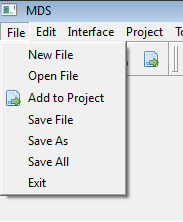
\includegraphics[width=.25\textwidth]{img/menu_file.png}
                &
            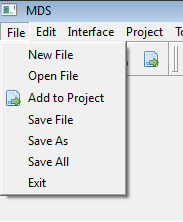
\includegraphics[width=.25\textwidth]{img/menu_file.png}
                &
            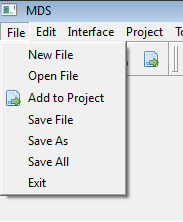
\includegraphics[width=.25\textwidth]{img/menu_file.png}
                \\
            Project selection & Edit selection & File selection
        \end{tabular}
    \end{table}

\subsection{Bottom panel}
    Here you can see bottom panel. You can see status of internal registers, scratchpad ram, input and output ports, stack, program counter, elapsed time and cycles, actual clock and internal flags: CARRY and ZERO. All those features can be edited during processor simulation. 

   \begin{figure}[h!]
        \centering
        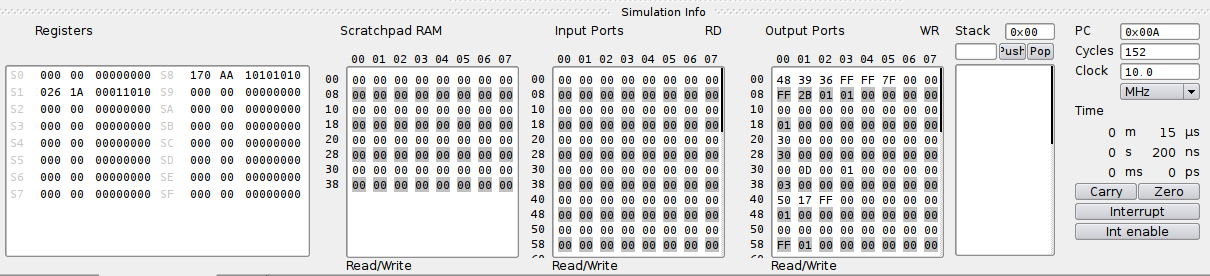
\includegraphics[width=\textwidth]{img/bottom_panel.png}
        \caption{Window layout concept}
    \end{figure}

\subsection{Right panel}
    Right panel contains list of breakpoints and bookmarks. Yoou can also find here list of symbols and macros in your source code.
\subsection{Left panel}

\clearpage
\enlargethispage{6\baselineskip}
\subsection{Project configuration}
    In project configuration window, you can edit project and compiler settings. You can open project configuration window by right clicking to project name in the left panel. See the pictures below.
    \begin{figure}[h]
        \centering{}
        
\includegraphics[width=.9\textwidth]{img/mensi_obrazek.png}
        \caption{Opening project configuration window from main screen.}
    \end{figure}

    This will open main configuration window with multiple tabs on the left side.
    \begin{figure}[h!]
        \centering{}
        
\includegraphics[width=.9\textwidth]{img/mensi_obrazek.png}
        \caption{Project window layout.}
    \end{figure}

    \clearpage

    \begin{itemize}
        \item Undo: will undo all edit actions on the open document in reverse order
        \item Redo: will redo all undo actions
        \item Cut: cuts all selected parts of the open doecument and puts it on the clipboard
        \item Copy: copies all selected parts of the open document to the clipboard
        \item Paste: pastes the text contents of the clipboard in the open document
        \item Select: All selects all text in the open document
        \item Find: find a to be given string through the open document
        \item Replace: replace a given string in the open document by a new string
    \end{itemize}

    \begin{itemize}
        \item Undo: will undo all edit actions on the open document in reverse order
        \item Redo: will redo all undo actions
        \item Cut: cuts all selected parts of the open doecument and puts it on the clipboard
        \item Copy: copies all selected parts of the open document to the clipboard
        \item Paste: pastes the text contents of the clipboard in the open document
        \item Select: All selects all text in the open document
        \item Find: find a to be given string through the open document
        \item Replace: replace a given string in the open document by a new string
    \end{itemize}

\section{Other tools}

\subsection{Code Completion list}
    The Code Completion List shows program symbols that contain the characters you are currently typing.
    \begin{figure}[h]
        \centering{}
        
\includegraphics[width=.3\textwidth]{img/mensi_obrazek.png}
        \caption{Code completion list}
    \end{figure}

\clearpage
\subsection{Parameter Information}
    Parameter Information shows the names, amount of, and parameter types of a function or method. The parameter in bold indicates the next parameter that is required as you are typing.
    \begin{figure}[h]
        \centering{}
        
\includegraphics[width=.3\textwidth]{img/mensi_obrazek.png}
        \caption{Parametr information list}
    \end{figure}

\subsection{DATA file convertor}
    This tool alows you to convert selected data file to another. Mutual conversion can be made with Hex, Bin, SRec, XilMem, XilVerilog and XilVhdl.
    \begin{description}
        \item[Section Input File] Here you can select desired input data file which is going to be converted
        \item[Section Input Options] In this section, you define what type of input file is going to be converted
        \item[Input file type] Available options - Hex, Bin, SRec, XilMem, XilVerilog and XilVhdl
        \item[Bytes per record] Only if you want to convert XilMem file. Defines number of bytes per record
        \item[OPCode size] Defines opcode size of selected data file. Available are 16 and 18
        \item[Section Output File] Defines target
        \item[Section Output Options] Here you can select desired output data file.
        \item[Input file type] Available options - Hex, Bin, SRec, XilMem, XilVerilog and XilVhdl.
        \item[Tab size]  Define number of inserted spaces when you press Tab.
        \item[Short instructions] Here you can allow short instructions like LD, RETI or others
    \end{description}

    \begin{figure}[h]
        \centering{}
        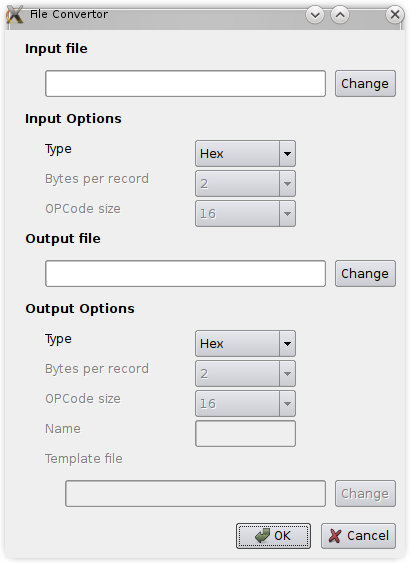
\includegraphics[width=.5\textwidth]{img/DATA_convertor.png}
        \caption{DATA file convertor}
    \end{figure}

\subsection{ASM translator}
    With this tool, you can translate your previously written assembler code in different syntax.
    You can sellect one of three choices - Xilinx, Mediatronix and OpenPicIde. Input code should be without
    errors.
    \begin{description}
        \item[Section Input File] Here you can choose which file you want to translate into the MDS assembler
        \item[Section ASM type] Input file syntax version. Translator needs to know input file syntax. Select one of three choices - Xilinx, Mediatronix and OpenPicIde
        \item[Symbol] Case of symbols - UPPERCASE or LOWERCASE
        \item[End of line] Indentation - Choose between Tabs or Spaces
        \item[Directive] Case of Directives - UPPERCASE or LOWERCASE
        \item[Indentation] Three choices - Tabs, Spaces and Keep (indentation unchanged)
        \item[Instruction] Case of instructions - UPPERCASE or LOWERCASE
        \item[Tab size]  Define number of inserted spaces when you press Tab.
        \item[Short instructions] Here you can allow short instructions like LD, RETI or others
    \end{description}

    \begin{figure}[h]
        \centering{}
        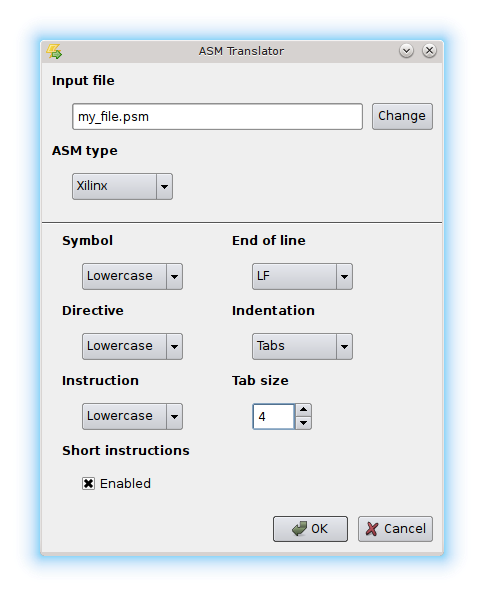
\includegraphics[width=.5\textwidth]{img/ASM_translator.png}
        \caption{ASM translator}
    \end{figure}

\subsection{Disassembler}
    A disassembler is a tool that translates machine language into assembly language. The inverse
    operation to that of an assembler.

    \begin{description}
        \item[Section File] Here you can choose which file you want to be disassembled
        \item[Section Target] Architecture - Select processor architecture
        \item[Family] select processor family of selected architecture
        \item[Section Options] Indentation - Choose between Tabs or Spaces
        \item[TabSize] Number of spaces in one tab
        \item[Radix] Binary,Octal, Decima or Hexadecimal
        \item[Linebreak] LF,CR or CRLF
        \item[Case]  You can choose if you want disassemled file will be in upper or lower case
        \item[Generate symbols] Select which symbols should be disassembled
    \end{description}

    \begin{figure}[h]
        \centering{}
        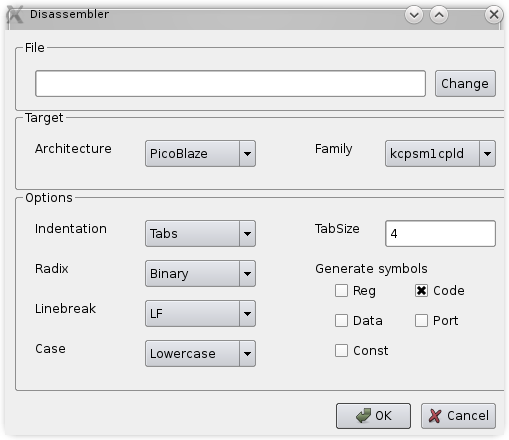
\includegraphics[width=.5\textwidth]{img/disassembler_window.png}
        \caption{Disassembler}
    \end{figure}

\subsection{Syntax Checking}
    Syntax Checking validates the program syntax while you are typing the code and provides real-time alerts to potential code violations before compilation. This enhances productivity and greatly reduces edit, compile, and correction cycles.
    \begin{figure}[h]
        \centering{}
        
\includegraphics[scale=0.3]{img/mensi_obrazek.png}
        \caption{Syntax checking picture}
    \end{figure}

\subsection{Instruction details}

\subsection{Subprograms call monitor}

\subsection{ASCII chart}

\subsection{PicoBlaze Instruction Table}

\subsection{Symbol viewer}

\subsection{Stopwatch}

\subsection{Hexadecimal editors}

\subsection{Interrupt monitor}

\subsection{8-segment editor}
    \begin{wrapfigure}{r}{0pt}
        \centering{}
        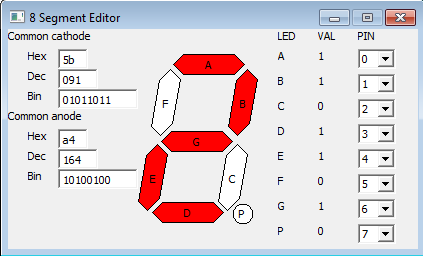
\includegraphics[width=110pt]{img/8segment.png}
        \caption{8-segment editor}
    \end{wrapfigure}
    With this tool you can easily determine what value you have to set on a port to display a digit on a numerical LED display. In the left part of the dialog window, you can find numerical val ues corresponding to the digit displayed in the middle part. These values are represented for both common cathode and anode and in three numerical bases, hexadecimal, decimal and oc tal. Buttons on left side from entry boxes copies value from adjacent entry box into clipboard. In the right part of the window you can set what port pin is connected to what LED segment.

\subsection{Number base converter}
    \begin{wrapfigure}{r}{0pt}
            \centering
            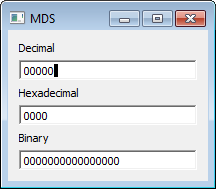
\includegraphics[width=90pt]{img/convertor.png}
            \caption{Convertor}
    \end{wrapfigure}
    This tool is very usefull, when you want to find out the representation of given number in other number bases.
